\documentclass{beamer}

\usepackage[utf8]{inputenc} 
\usepackage[T1]{fontenc}
\usepackage{lmodern}
\usepackage{graphicx}
\usepackage[french]{babel}
\usepackage{tikz}
\usetikzlibrary{arrows,shapes,positioning}


\frenchbsetup{StandardLists=true}
\usetheme{Singapore}
\setbeamertemplate{navigation symbols}{} 
\author{Julien Deguilhem\and Maïlys Denis\and Sébastien Gautheron\and Johann Mitrail\and Anthony Rossi\and Colin Vidal}
\date{}

\setbeamertemplate{footline}{
\begin{beamercolorbox}[]{section in head/foot}
\begin{center}
\insertframenumber{} / \inserttotalframenumber\hspace*{2ex}
\end{center}
\end{beamercolorbox}
}
 
\begin{document}
 
\title{Projet Thésaurus}
\maketitle


\frame{
\frametitle{Introduction}
\begin{itemize}
\item Définition d'un thésaurus
\item Organisation du groupe
\item Modélisation
\item Implémentation
\end{itemize}
}


\begin{frame}
\frametitle{Qu'est ce qu'un thésaurus ?}
trouver def pas trop pompeuse... ce diapo est vraiment utile ? peut-être plutot dire que le notre sera sur les animaux serait mieux 
\end{frame}



\begin{frame}
\frametitle{Organisation du projet}
\begin{itemize}
\item réunions tous les 15 jours
\item contacts réguliers par mail
\item gestion des sources via un dépôt Git
\end{itemize}
\end{frame}


\begin{frame}
\frametitle{Répartition des tâches}
\begin{itemize}
\item Julien : implémentation web
\item Colin : infrastructure + modélisation + implémentation BDD
\item Sébastien : réalisation de diagrammes
\item Anthony : chef de projet + design site web
\item Johann : rapport
\item Maïlys : implémentation web  + rapport
\end{itemize}
\end{frame}


\begin{frame}
\frametitle{Modélisation}
Deux modèles de stockage des données ont étés envisagés
\begin{itemize}
\item sous forme d'arbre
\item sous forme de graphe orienté
\end{itemize}
\end{frame}


\begin{frame}
\frametitle{Modèle sous forme d'arbre}
\begin{center}
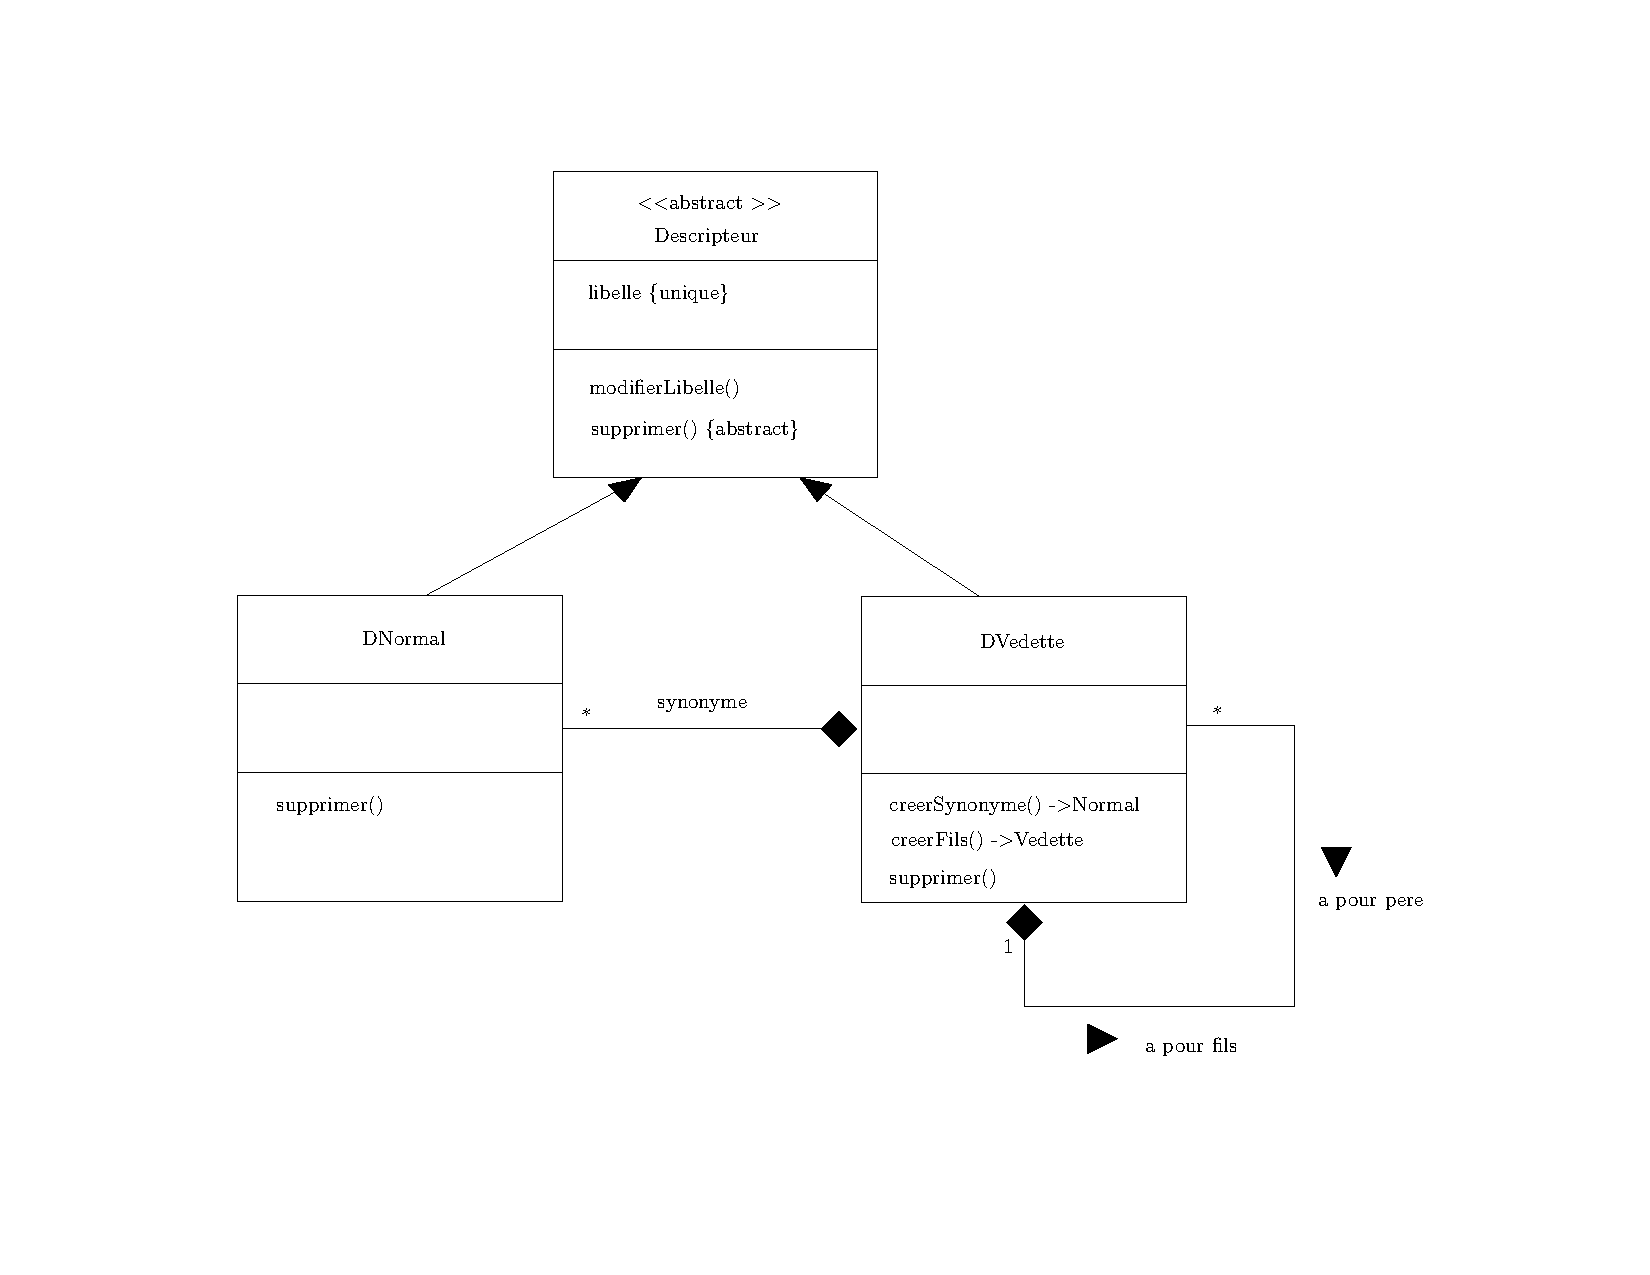
\includegraphics[width=8cm, trim = 0cm 2cm 2cm 2cm, clip=true]{diag_de_classe_old.pdf}
\end{center}
\begin{itemize}
\item trop spécifique
\item ne supporte pas l'héritage multiple
\item opérations de suppression délicates en objet
\end{itemize}
\end{frame}


\begin{frame}
\frametitle{Modèle sous forme de graphe orienté}
\begin{center}
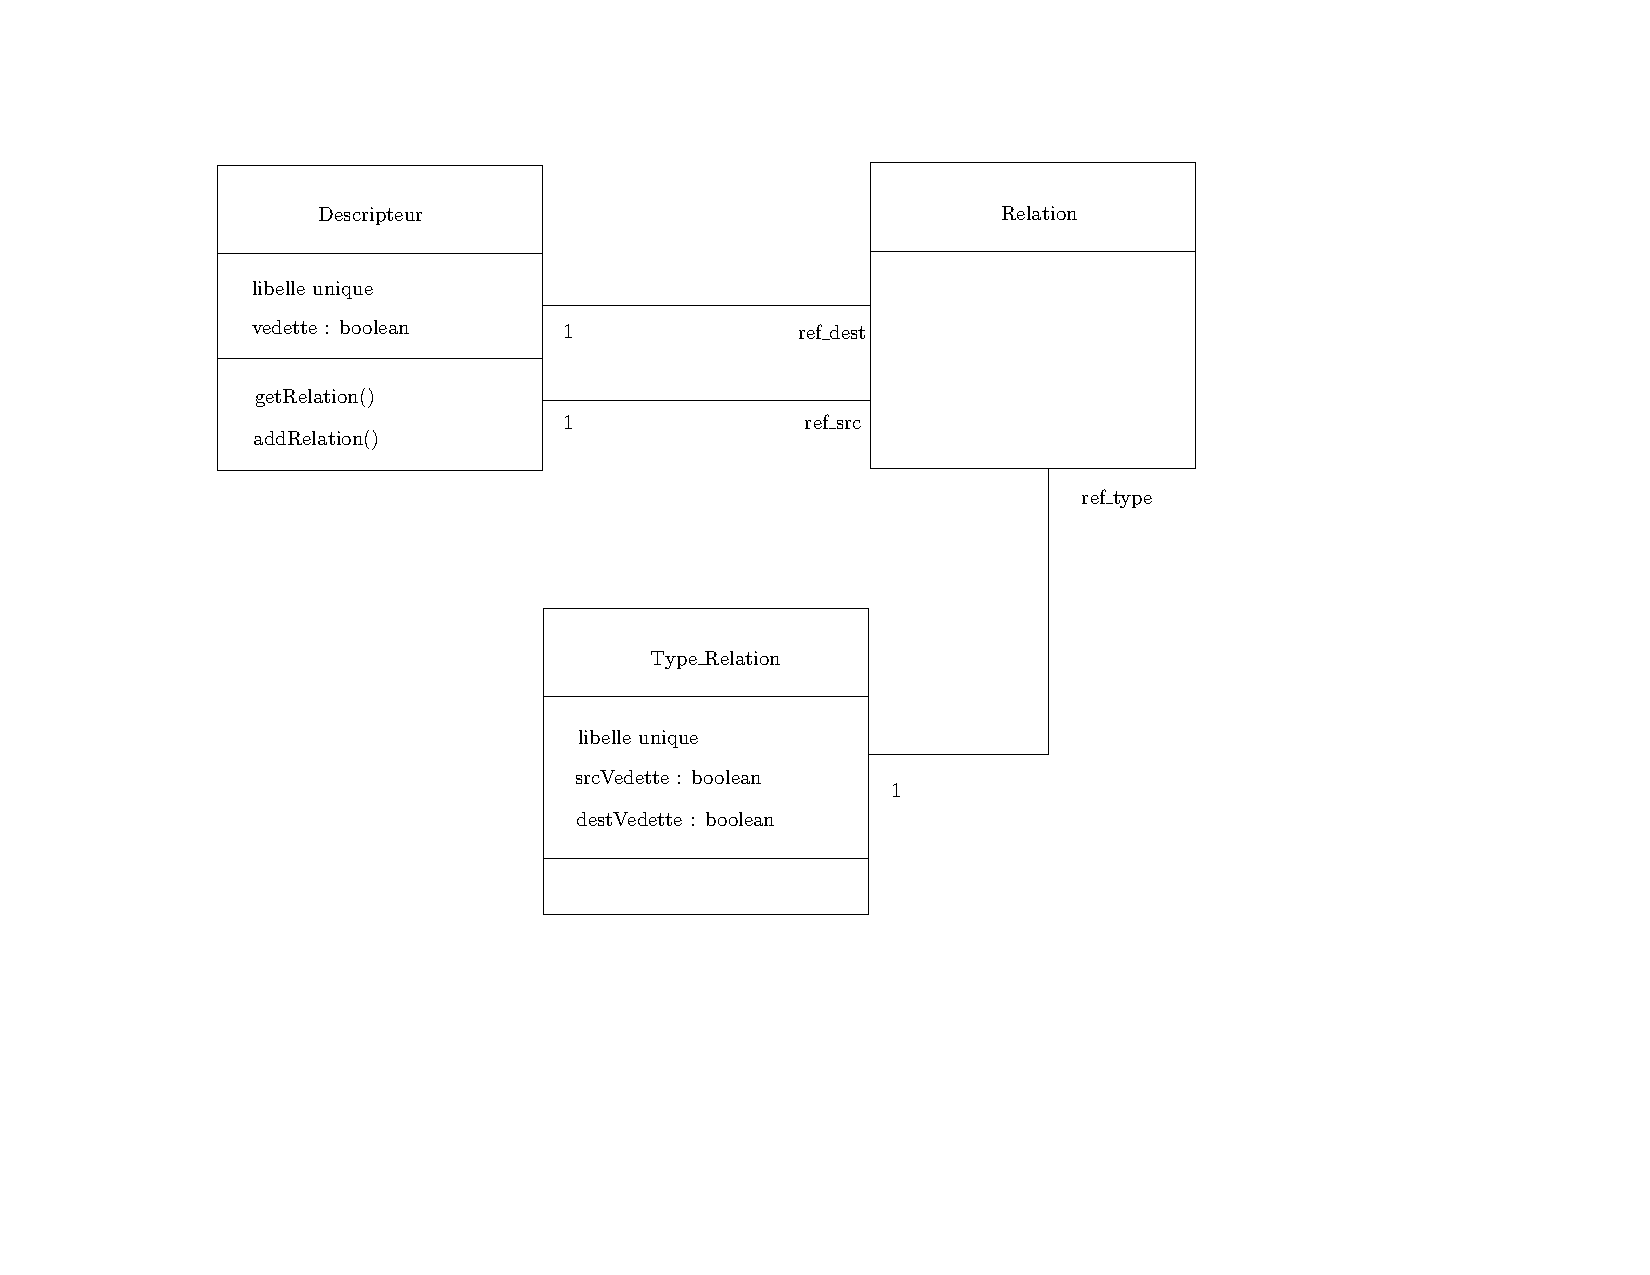
\includegraphics[width=12cm]{diag_de_classe.pdf}
\end{center}
\begin{itemize}
\item trop spécifique
\item ne supporte pas l'héritage multiple
\item opérations de suppression délicates en objet
\end{itemize}
\end{frame}


\begin{frame}
\frametitle{Modèle sous forme de graphe orienté}
\begin{itemize}
\item très généraliste et souple à manipuler
\item triggers pour assurer les contraintes de relations (vedette/non vedette)
\item risque de lenteur sur de gros volumes de données/insertions simultanées multiples
\item une relation correspond à un triplet descripteur source, descripteur destination, type relation
\end{itemize}
\end{frame}


\begin{frame}
\frametitle{Infrastructure}
\begin{itemize}
\item Oracle 11g
\item Apache2 + PHP + OCI
\item MV KVM sous CentOS récupérant la dernière version des sources régulièrement
\end{itemize}
\end{frame}



\begin{frame}
\frametitle{Implémentation base de données}
\begin{itemize}
\item Une relation associe deux descripteurs et un type de relation par les références des objets des tables Descripteurs et Type\_Relations (vue objet relationnelle)
\item Déclencheurs (ajout/modification table Relations)
\begin{itemize}
\item unicité triplet réf. desc. source, réf. desc. destination, réf. type relation (impossible d'utiliser les références comme clé primaire)
\item cohérence des associations en fonction du type de relation\\ (ex. relation de type \emph{Synonyme} doit avoir un descripteur source vedette et descripteur destination non vedette)
\end{itemize}
\end{itemize} 
\end{frame}


\begin{frame}
\frametitle{Implémentation web}
\begin{itemize}
\item Classe Descripteur
\begin{itemize}
\item recherche de descripteur / relation
\item ajout de descripteur
\item ajout de relation
\item suppression de relation (non implémenté dans l'interface utilisateur)
\end{itemize}
\item Simplification des URL (module rewrite Apache + htaccess)\\ \emph{domain.tld/index.php?lib=chat} $\rightarrow$ \emph{domain.tld/chat/}
\end{itemize}
\end{frame}


\begin{frame}
\frametitle{Interface utilisateur}
\begin{itemize}
\item design CSS + HTML (Bootstrap)
\item 2 pages principales
\begin{itemize}
\item beuuu
\end{itemize}
\end{itemize}
\end{frame}


\begin{frame}
\frametitle{Conclusion}

\end{frame}

\end{document}
